\section{Adaptive Estimation \label{sec:sequential}}

The first main result of this paper (Theorem~\ref{thm:adpative_lower_bound})
gives that the asymptotic variance of any adaptive estimator must be at
least $\eta(0)\sigma^2$, which is precisely the efficiency of the median of
the sample $X_1,\ldots,X_n$. Conveniently, the stochastic (sub)gradient
estimator for the median---which minimizes $\E[|X - \theta|]$---is a
sequence of signs (single bits), so that we can exhibit an asymptotically
optimal adaptive estimation scheme.

%Finally, in Theorem~\ref{thm:opt_one_step}, we provide an adaptive estimation scheme that is one-step optimal in the sense that at each step $i$, the chosen message $B_i$  minimizes the MSE given $X_i$ and the previous $i-1$ messages. %Numerical simulations for the case of $f(x)$ the normal density function shows that the ARE of the estimator described by this scheme is $\eta(0)\sigma^2$. 

We begin with our first theorem, whose proof we provide in
Appendix~\ref{proof:thm:adpative_lower_bound}.
\begin{thm}[Fundamental limits]\label{thm:adpative_lower_bound}
  Let Assumption~\ref{assump:failure_rate} hold.
  Let ${\theta}_n$ be any estimator of $\theta$ in the adaptive setting of
  Figure~\ref{fig:setup}(ii). Assume that the prior
  density $\pi(\cdot)$ on $\theta$ converges to zero
  at the endpoints of the interval $\Theta$ and
  define the prior Fisher information
  $I_0 \defeq \E_\pi[(\pi'(\theta) / \pi(\theta))^2]$.
  Then
  \begin{equation*}
    n \E\left[ (\theta-{\theta}_n)^2 \right] \geq   \frac{n}{ 4f^2(0) n + I_0}.
  \end{equation*}
\end{thm}

%We first bound from above the Fisher information of any set of $n$ one-bit messages with respect to $\theta$. The result then follows using the van-Trees inequality which bounds from below the risk of any estimator of $\theta$ by the inverse of the expected value of the aforementioned Fisher information plus $I_0$. The details are in

%% Theorem~\ref{thm:adpative_lower_bound} implies that any estimator ${\theta}_n$ from any adaptive encoding scheme satisfies
%% \begin{equation*}
%% n\mathbb E\left[ (\theta-\theta_n)^2 \right] \geq  \frac{1}{4f^2(0)}+O(n^{-1}),
%% \end{equation*}
%% and 
%% \begin{equation*}
%% \ARE({\theta}_n) \leq 4f^2(0)\sigma^2 = \eta(0)\sigma^2.
%% \end{equation*}
It is possible to extend Theorem~\ref{thm:adpative_lower_bound} to any other
loss functions using a more subtle version of the Van Trees
inequality~\cite{efroimovich1980information}; see also
\cite{DBLP:journals/corr/abs-1902-08582}.

We now turn to asymptotically optimal estimators, first
showing how a simple stochastic gradient scheme is asymptotically
optimal (in the fully adaptive setting), after which we show that
a one-round adaptive scheme can also achieve this optimal efficiency.

\subsection{Asymptotically optimal estimator}

The starting point for our first estimator is to note that the median of a
distribution minimizes $\E[|X - \theta|]$ over $\theta \in \R$, and
moreover, we have the familiar result (cf.~\cite{VanDerVaart98}, Ch.~21)
that given a sample $X_1^n \simiid P$, if $\theta = \mbox{med}(P)$ and
$P$ has continuous density $f(\cdot - \theta)$ near $\theta$, then
\begin{equation*}
  \sqrt{n}(\mbox{med}(X_1^n) - \theta)
  \cd \normal\left(0, \frac{1}{4 f(0)^2}\right),
\end{equation*}
which is precisely the variance lower bound in
Theorem~\ref{thm:adpative_lower_bound}.  Thus, it it is natural consider a
stochastic gradient procedure for minimizing $\E[|X - \theta|]$. To that end,
let $\left\{ \gamma_n \right\}_{n\in \mathbb N}$ be a strictly positive
sequence of stepsizes,
and define the sequence
\begin{equation}
  \label{eq:sgd_alg}
  \theta_n = \theta_{n-1} + \gamma_n B_n, \quad n = 1,2,\ldots,
\end{equation}
where 
\begin{equation*}
  B_n = \sgn (X_n - \theta_{n-1}).
\end{equation*}
We make one of two assumptions on the stepsizes $\gamma_n$, which
are relatively standard: we always have $\gamma_n$ non-increasing, and
\begin{subequations}
  For some $0 < \lambda \le 1$,
  \begin{align}
    \label{eqn:lazy-gamma}
    \frac{\gamma_n - \gamma_{n+1}}{\gamma_n^2}
    \to 0, & ~~~
    \sum_n \frac{\gamma_n^\frac{1 + \lambda}{2}}{\sqrt{n}} < \infty
    ~~ \mbox{or} \\
    \gamma_n = o(n^{-2/3}),
    & ~~~
    \sum_n \gamma_n = \infty.
    \label{eqn:stringent-gamma}
  \end{align}
\end{subequations}

Then we can adapt the results of Polyak and Juditsky~\cite{PolyakJu92}
on the asymptotic normality of averaged stochastic gradient estimators
to establish the following theorem.
\begin{thm}
  \label{thm:sgd}
  Define the average $\bar{\theta}_n \defeq \frac{1}{n}
  \sum_{i = 1}^n \theta_i$. Assume
  that in a neighborhood
  of $\theta = \mbox{med}(P)$,
  the distribution $P$ has a Lipschitz continuous density $f$.
  Then
  \begin{enumerate}[(i)]
  \item \label{item:normal-sgd}
    Assume that $\left\{ \gamma_n \right\}_{n\in \mathbb N}$ satisfies
    condition~\eqref{eqn:lazy-gamma}.
    Then
    \begin{equation*}
      \sqrt{n}\left( \bar{\theta}_n - \theta\right)
      \cd \normal\left(0,\frac{1}{4 f(\theta)^2}\right).
    \end{equation*}
    %
    %
  \item \label{item:sgd-regular}
    %(or that $f(x-\theta)$ is differentiable in quadratic mean).  
    For any bounded, symmetric, and quasi-convex function $L$, 
    \begin{align} 
      & \sup_{c < \infty} \limsup_{n \to \infty}
      \sup_{\tau\,:\,|\theta-\tau| \leq \frac{c}{\sqrt{n} }}
      \E_\tau \left[ L\left( \sqrt{n}(\bar{\theta}_{n} - \tau) \right) \right] \nonumber 
      \\
      & \qquad \qquad \qquad \qquad = \mathbb E \left[L(W/ 2 f(0)) \right],
        \label{eq:attaining_LAM}
    \end{align}
    where $W \sim \normal(0,1)$. 
    %
    %
  \item \label{item:sgd-ms-convergence}
    Assume the stepsizes $\gamma_n$ satisfy both
    conditions~\eqref{eqn:lazy-gamma} and~\eqref{eqn:stringent-gamma}.
    Then
    \begin{equation*}
      \ex{\left( \bar{\theta}_n - \theta \right)^2} = \frac{1}{4 n f(\theta)^2} + o(n^{-1}). 
    \end{equation*}
  \end{enumerate}
\end{thm}

\noindent
We provide the proof in Appendix~\ref{proof:sgd}.

As an immediate corollary to Theorem~\ref{thm:sgd}, we obtain the following
asymptotic optimality results of the averaged stochastic gradient
sequence.
%% \begin{corollary}

\textbf{FILL THIS IN}

%% \end{corollary}

Theorem~\ref{thm:sgd} implies that the estimator ${\theta}_n$ defined by \eqref{eq:sgd_est} and \eqref{eq:sgd_alg} attains the maximal ARE, as established by Theorem~\ref{thm:adpative_lower_bound}. %Furthermore, it is locally minimax in the sense that it attains the minimal MSE for all local alternatives of $\theta$. 
%
The update step \eqref{eq:sgd_alg} can be seen as a gradient descent step for the function $x\to |x|$ at the point $x=X_n - \theta_{n-1}$. Consequently, the procedure above is known as averaged stochastic gradient descent for minimizing $x \to |x|$ given the data $X_1,\ldots,X_n$. The minimal value of this optimization is the sample median, and Theorem~\ref{thm:sgd} provides conditions for the sequence of gradient steps so that the algorithm converges to this minimum. In particular, parts (i) and (ii) of Theorem~\ref{thm:sgd} provides conditions under which $\bar{\theta}$ is asymptotically normal and local asymptotically minimax, in the sense that it attains the local asymptotic minimax bound \cite{van2000asymptotic}. Part (iii) provides an additional condition under which $\bar{\theta}$ also converges in its second moment. 
 \par
%Note that $\theta_0$ is not explicitly defined in equation \eqref{eq:sgd_est}. A reasonable initialization for $\theta_0$ is $\theta_0 = \mathbb E [\theta]$, although Theorem~\ref{thm:sgd} implies that the asymptotic behavior of the estimator is indifferent to this initialization. Thus, the optimal efficiency is attained regardless of the prior distribution on $\theta$ or the radius of the parameter space $\Theta$.  \\
In the encoding and estimating procedure \eqref{eq:sgd_alg} and \eqref{eq:sgd_est}, each one-bit message $B_n$ depends on its private sample as well as the current gradient descent estimate $\theta_{n-1}$. In this sense, each encoder in this algorithm interacts with previous one by using the current estimate.
%
As we explain next, 
it is possible to obtain the optimal efficiency of $\eta(0)\sigma^2$ with only one round of interactions among the encoders. 


%% \begin{figure}
%% \begin{center}
%% \begin{tikzpicture}[node distance=2cm,auto]
%%   \node at (0,0) (source) {$X_1$} ;
%%   \node[int1, right of = source, node distance = 1.2cm] (enc1) {$\enc$};  
%% \draw[->,line width = 2pt] (source) -- (enc1); 

%% % \node[below of = source, node distance = 1cm] (source2) {$X_2$};
%% %\node[int1, right of = source2, node distance = 1.2cm] (enc2) {Enc};  
%% %\draw[->,line width = 2pt] (source2) -- (enc2); 

%% \node[below of = source, node distance = 1.7cm] (source3) {$X_{n_1}$};
%% \node[int1, right of = source3, node distance = 1.2cm] (enc3) {$\enc$};  

%% \draw[->,line width = 2pt] (source3) -- (enc3); 

%% \node[below of = source, node distance = 0.5cm] {$\vdots$};

%% \node[int1, right of = enc3, node distance = 2.1cm ] (est) {$\est_1$};

%% \draw[->,line width = 2pt] (enc1) -| node[above, xshift = -1cm] (mes1) {$B_1$} (est);   

%% %\draw[->,line width = 2pt] (enc2) -| node[above, xshift = -1cm] (mes2) {$B_2$} (est);   

%% \draw[->,line width = 2pt] (enc3) -- node[above, xshift = 0cm]  {$B_{n_1}$} (est);   

%% \node[below right = 0.75 and 1.5 of source3] (sourceB) {$X_{n_1 +1}$} ;
%% \node[int1, right of = sourceB, node distance = 1.7cm] (enc1B) {$\enc$};  
%% \draw[->,line width = 2pt] (sourceB) -- (enc1B); 

%% \node[below of = sourceB, node distance = 1.7cm] (source3B) {$X_n$};
%% \node[int1, right of = source3B, node distance = 1.7cm] (enc3B) {$\enc$};  
%% \draw[->,line width = 2pt] (source3B) -- (enc3B); 
%% \node[below of = sourceB, node distance = 0.4cm] {$\vdots$};

%% \node[int1, right of = enc3B, node distance = 2.1cm ] (estB) {$\est_2$};

%% \draw[->,line width = 2pt] (enc1B) -| node[above, xshift = -0.5cm] {$B_{n_1+1}$} (estB);
%% \draw[->,line width = 2pt] (enc3B) -- node[above] {$B_n$} (estB);

%% \draw[->,line width = 1pt] (est.east) node[above, xshift  =0.5cm] {${\theta}_{n_1}$} -| (enc1B.north);

%% %\draw[->,line width = 1pt] (enc1B) -- (enc3B);

%% \draw[->,line width = 0.5pt] (est.east) -| +(1.3,-0.5) -- +(1.3,-2.5) -| (enc3B.north);

%% %\draw[->,line width = 1pt] (enc1B)  -- node[right] {${\theta}_{n_1}$} (enc3B);

%% \draw[->,line width = 0.5pt] (estB) -- +(0.8,0) node[right] {${\theta}_n$};
%% \node[below of = enc1B, node distance = 0.5cm] {$\vdots$};

%% \end{tikzpicture}
%% \end{center}
%% \caption{Distributed encoding with a single interaction: The estimation obtained from the first $n_1$ bits in a distributed manner is to obtain another $n-n_1$ bits in a distributed manner. 
%% \label{fig:one_round}
%% }
%% \end{figure}

\subsection{Maximal Efficiency using One Round of Threshold Adaptation}
In Section~\ref{sec:preliminary} we considered an estimator that is based on binary messages of the form 
\begin{equation*}
B_i = \mathbf 1_{X_i > \theta_0},\qquad i=1,\ldots,n,
\end{equation*}
and deduced that it is asymptotically normal with variance $1/\eta(\theta-\theta_0)$.
%
We now show that a similar encoding leads to an asymptotically normal estimator attaining the lower variance bound $1/\eta(0)$, provided we allow to  update the threshold value $\theta_0$ based on previously observed bits at least once. 
%
In this procedure we separate the sample into two disjoint sets: $X_1,\ldots,X_{n_1}$ and $X_{n_1+1},\ldots,X_n$ for some $n_1 < n$.
We first use the estimator \eqref{eq:estimator_naive} to obtain an estimate ${\theta}_{n_1}$ based on $B_1,\ldots,B_{n_1}$, and then use ${\theta}_{n_1}$ as the new threshold value to obtain messages $B_{n_1+1}, \ldots, B_n$. Figure~\ref{fig:one_round} illustrates a diagram of this procedure. 
%
The specific encoding and estimation scheme, as well as its asymptotic performance, are given by the following theorem:
\begin{thm}
For $i=1,\ldots,n$ set
\begin{equation*}
B_i = \begin{cases}
 \mathbf 1_{X_i \geq \theta_0} & i = 1,\ldots,n_1, \\
 \mathbf 1_{X_i \geq {\theta}_{n_1} }& i={n_1+1,\ldots,n},
\end{cases}
\end{equation*}
where $n = n_1+ n_2$ and 
\begin{equation*}
{\theta}_{n_1} \triangleq \theta_0 + F^{-1}\left(
\frac{1}{n_1} \sum_{i=1}^{n_1} B_i 
 \right).
\end{equation*} 
Let 
\begin{equation*}
{\theta}_{n_2}  \triangleq {\theta}_{n_1} +  F^{-1} \left( \frac{1}{n_2} \sum_{i=n_1+1}^{n_2} B_i \right)
\end{equation*}
and assume that, as $n\to \infty$, $n_1(n) \rightarrow \infty$ and $n_2(n)/n \rightarrow 1$. Then:
\begin{align*}
 \sqrt{n} \left( {\theta}_{n_2} - \theta  \right) \overset{d}{\longrightarrow}  \Ncal\left( 0, 1/\eta(0) \right).
\end{align*}
\end{thm}
%
%
\begin{proof}
For $t\in \mathbb R$, set
\begin{equation*}
p_{n_2}(t) \triangleq \frac{1}{n_2} \sum_{i=n_1+1}^{n} \mathbf 1_{X_i \geq t}. 
\end{equation*}
Since $n_2(n)/n \to 1$, if follows from the Berry Esseen theorem that there exists $C$, independent of $n$ and $t$, such that 
\begin{align*}
\sup_{t \in \R} \left| \sqrt{n} \frac{ p_{n_2}(t) - F( \theta - t)} {F(\theta - t) F \left( t - \theta\right) }  - \Phi(t) \right|  \leq C/\sqrt{n}. 
\end{align*}
where $Z \sim \Ncal(0,1)$. It follows that
\begin{align}
\label{eq:two_step_proof}
 \sqrt{n} \frac{ p_{n_2}(Y_n) - F(0)} {F^2(0) }  \overset{d}{\rightarrow} \Ncal(0,1)
\end{align}
for any sequence of random variables $\{Y_n\}$ converging in probability to $\theta$. In particular, since
\begin{equation*}
p_{n_1} \triangleq \frac{1}{n_1} \sum_{i=1}^{n_1} B_i \overset{a.s.}{\rightarrow} F(\theta - \theta_0)
\end{equation*}
by the law of large numbers, \eqref{eq:two_step_proof} holds for $Y_n = \theta_{n_1}$. Finally, we use the delta method with $g(x) = F^{-1}(x)$ to conclude
\begin{align*}
& \sqrt{n}\left( \theta_{n_2} - \theta \right) = \sqrt{n} \left( \theta_{n_1} + F^{-1}(p_{n_2}(\theta_{n_1})) - \theta \right) \\
&= \sqrt{n} \left( g(p_{n_2}(\theta_{n_1})) - g \left(F(\theta-\theta_{n_1}) \right)  \right) \overset{d}{\to} \Ncal\left(0, 
F^2(0)/ f^2(0) \right).
\end{align*}
\end{proof}
%

%% \begin{figure}
%% \begin{center}
%% \begin{tikzpicture}[scale = 0.6]
%% \begin{axis}[
%% width=10cm, height=6cm,
%% xmin = 0, xmax=800, 
%% restrict y to domain = 0:3,
%% ymin = 0,
%% ymax = 3.4,
%% samples=10, 
%% xlabel= $n$,
%% ylabel = {$n\mathbb E \left[\left(\theta - {\theta}_n \right)^2 \right]$},
%% %xtick={-3,-2,-1,0,1,2,3},
%% %xticklabels={-3,-2,-1,0,1,2,3},
%% ytick={0,1,1.57},
%% yticklabels={0,1,$\pi/2$},
%% line width=1.0pt,
%% mark size=1.5pt,
%% ymajorgrids,
%% xmajorgrids,
%% legend style= {at={(1,1)},anchor=north east,draw=black,fill=white,align=left}
%% ]

%% \addplot[color = blue, solid, smooth] plot table [x = itr, y = SGD, col sep=comma] {./SimRes/sim_res_nMonte5000.csv};
%% \addlegendentry{asymptotically optimal};

%% %\addplot[color = red, solid, smooth] plot table [x = itr, y = Bayes, col sep=comma] {./SimRes/sim_res_nMonte5000.csv};\addlegendentry{one step optimal};

%% \addplot[color = red, solid, smooth] plot table [x = itr, y = split, col sep=comma] {./SimRes/sim_res_nMonte5000.csv};
%% \addlegendentry{single interaction};

%% \end{axis}
%% \end{tikzpicture}
%% %\begin{tikzpicture}
%% %\node at (0,0) {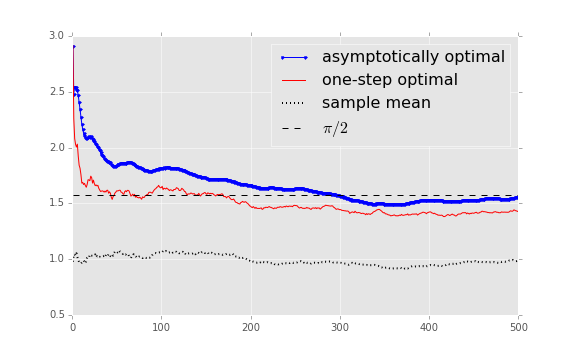
\includegraphics[scale=0.4]{one_bit_adpative}};
%% %\node[rotate = 90, scale = 0.7] at (-3.8,0) {$n \mathbb E \left({\theta}_n - \theta \right)^2$};
%% %\node[scale = 0.7] at (0,-2.4) {$n$};
%% %\end{tikzpicture}
%% \caption{Normalized empirical risk versus number of samples $n$ for $10,000$ Monte Carlo trials with $f(x)$ the standard normal density. In each trial, $\theta$ is chosen uniformly over the interval $(-1.64,1.64)$. The single interaction strategy uses $n_1 = \lfloor \sqrt{n} \rfloor$ samples for its first stage. 
%% \label{fig:adaptive_error}  }
%% \end{center}
%% \end{figure}
